% Options for packages loaded elsewhere
\PassOptionsToPackage{unicode}{hyperref}
\PassOptionsToPackage{hyphens}{url}
%
\documentclass[
]{article}
\usepackage{amsmath,amssymb}
\usepackage{lmodern}
\usepackage{iftex}
\ifPDFTeX
  \usepackage[T1]{fontenc}
  \usepackage[utf8]{inputenc}
  \usepackage{textcomp} % provide euro and other symbols
\else % if luatex or xetex
  \usepackage{unicode-math}
  \defaultfontfeatures{Scale=MatchLowercase}
  \defaultfontfeatures[\rmfamily]{Ligatures=TeX,Scale=1}
\fi
% Use upquote if available, for straight quotes in verbatim environments
\IfFileExists{upquote.sty}{\usepackage{upquote}}{}
\IfFileExists{microtype.sty}{% use microtype if available
  \usepackage[]{microtype}
  \UseMicrotypeSet[protrusion]{basicmath} % disable protrusion for tt fonts
}{}
\makeatletter
\@ifundefined{KOMAClassName}{% if non-KOMA class
  \IfFileExists{parskip.sty}{%
    \usepackage{parskip}
  }{% else
    \setlength{\parindent}{0pt}
    \setlength{\parskip}{6pt plus 2pt minus 1pt}}
}{% if KOMA class
  \KOMAoptions{parskip=half}}
\makeatother
\usepackage{xcolor}
\usepackage[margin=1in]{geometry}
\usepackage{color}
\usepackage{fancyvrb}
\newcommand{\VerbBar}{|}
\newcommand{\VERB}{\Verb[commandchars=\\\{\}]}
\DefineVerbatimEnvironment{Highlighting}{Verbatim}{commandchars=\\\{\}}
% Add ',fontsize=\small' for more characters per line
\usepackage{framed}
\definecolor{shadecolor}{RGB}{248,248,248}
\newenvironment{Shaded}{\begin{snugshade}}{\end{snugshade}}
\newcommand{\AlertTok}[1]{\textcolor[rgb]{0.94,0.16,0.16}{#1}}
\newcommand{\AnnotationTok}[1]{\textcolor[rgb]{0.56,0.35,0.01}{\textbf{\textit{#1}}}}
\newcommand{\AttributeTok}[1]{\textcolor[rgb]{0.77,0.63,0.00}{#1}}
\newcommand{\BaseNTok}[1]{\textcolor[rgb]{0.00,0.00,0.81}{#1}}
\newcommand{\BuiltInTok}[1]{#1}
\newcommand{\CharTok}[1]{\textcolor[rgb]{0.31,0.60,0.02}{#1}}
\newcommand{\CommentTok}[1]{\textcolor[rgb]{0.56,0.35,0.01}{\textit{#1}}}
\newcommand{\CommentVarTok}[1]{\textcolor[rgb]{0.56,0.35,0.01}{\textbf{\textit{#1}}}}
\newcommand{\ConstantTok}[1]{\textcolor[rgb]{0.00,0.00,0.00}{#1}}
\newcommand{\ControlFlowTok}[1]{\textcolor[rgb]{0.13,0.29,0.53}{\textbf{#1}}}
\newcommand{\DataTypeTok}[1]{\textcolor[rgb]{0.13,0.29,0.53}{#1}}
\newcommand{\DecValTok}[1]{\textcolor[rgb]{0.00,0.00,0.81}{#1}}
\newcommand{\DocumentationTok}[1]{\textcolor[rgb]{0.56,0.35,0.01}{\textbf{\textit{#1}}}}
\newcommand{\ErrorTok}[1]{\textcolor[rgb]{0.64,0.00,0.00}{\textbf{#1}}}
\newcommand{\ExtensionTok}[1]{#1}
\newcommand{\FloatTok}[1]{\textcolor[rgb]{0.00,0.00,0.81}{#1}}
\newcommand{\FunctionTok}[1]{\textcolor[rgb]{0.00,0.00,0.00}{#1}}
\newcommand{\ImportTok}[1]{#1}
\newcommand{\InformationTok}[1]{\textcolor[rgb]{0.56,0.35,0.01}{\textbf{\textit{#1}}}}
\newcommand{\KeywordTok}[1]{\textcolor[rgb]{0.13,0.29,0.53}{\textbf{#1}}}
\newcommand{\NormalTok}[1]{#1}
\newcommand{\OperatorTok}[1]{\textcolor[rgb]{0.81,0.36,0.00}{\textbf{#1}}}
\newcommand{\OtherTok}[1]{\textcolor[rgb]{0.56,0.35,0.01}{#1}}
\newcommand{\PreprocessorTok}[1]{\textcolor[rgb]{0.56,0.35,0.01}{\textit{#1}}}
\newcommand{\RegionMarkerTok}[1]{#1}
\newcommand{\SpecialCharTok}[1]{\textcolor[rgb]{0.00,0.00,0.00}{#1}}
\newcommand{\SpecialStringTok}[1]{\textcolor[rgb]{0.31,0.60,0.02}{#1}}
\newcommand{\StringTok}[1]{\textcolor[rgb]{0.31,0.60,0.02}{#1}}
\newcommand{\VariableTok}[1]{\textcolor[rgb]{0.00,0.00,0.00}{#1}}
\newcommand{\VerbatimStringTok}[1]{\textcolor[rgb]{0.31,0.60,0.02}{#1}}
\newcommand{\WarningTok}[1]{\textcolor[rgb]{0.56,0.35,0.01}{\textbf{\textit{#1}}}}
\usepackage{graphicx}
\makeatletter
\def\maxwidth{\ifdim\Gin@nat@width>\linewidth\linewidth\else\Gin@nat@width\fi}
\def\maxheight{\ifdim\Gin@nat@height>\textheight\textheight\else\Gin@nat@height\fi}
\makeatother
% Scale images if necessary, so that they will not overflow the page
% margins by default, and it is still possible to overwrite the defaults
% using explicit options in \includegraphics[width, height, ...]{}
\setkeys{Gin}{width=\maxwidth,height=\maxheight,keepaspectratio}
% Set default figure placement to htbp
\makeatletter
\def\fps@figure{htbp}
\makeatother
\setlength{\emergencystretch}{3em} % prevent overfull lines
\providecommand{\tightlist}{%
  \setlength{\itemsep}{0pt}\setlength{\parskip}{0pt}}
\setcounter{secnumdepth}{5}
\ifLuaTeX
  \usepackage{selnolig}  % disable illegal ligatures
\fi
\IfFileExists{bookmark.sty}{\usepackage{bookmark}}{\usepackage{hyperref}}
\IfFileExists{xurl.sty}{\usepackage{xurl}}{} % add URL line breaks if available
\urlstyle{same} % disable monospaced font for URLs
\hypersetup{
  pdftitle={Final Project},
  pdfauthor={Matthew Bentham},
  hidelinks,
  pdfcreator={LaTeX via pandoc}}

\title{Final Project}
\author{Matthew Bentham}
\date{2023-04-30}

\begin{document}
\maketitle

\hypertarget{energy-demand-victoria}{%
\section{Energy Demand Victoria}\label{energy-demand-victoria}}

\hypertarget{math1318-final-project}{%
\subparagraph{\texorpdfstring{MATH1318: Final Project
\n\n}{MATH1318: Final Project }}\label{math1318-final-project}}

Matthew Bentham 3923076 \n John Murrowood 3923075 \n

\begin{center}\rule{0.5\linewidth}{0.5pt}\end{center}

\hypertarget{contents}{%
\section{Contents}\label{contents}}

\hypertarget{introduction}{%
\section{1. Introduction}\label{introduction}}

With the resurrection of the SEC , announcement of offshore wind farms
in south east Victoria and Victoria's renewable energy target of 50\% by
2030, being able to accurately predict energy demand on a continual
basis is becoming more and more important. As renewable energy sources
like wind and solar do not produce constant energy outputs, accurate
forecasting of energy demand throughout the day is essential to ensure
renewable energy sources are utilized efficiently. Although demand
forecasting is increasingly relevant when incorporating renewable into
the grid, demand forecasting in general reduces over and underproduction
of energy and minimizes energy waste as a whole.

\textbf{Data
Source:}\url{https://www.kaggle.com/datasets/aramacus/electricity-demand-in-victoria-australia}

This data set contains the total daily energy demand across Victoria in
MWh from 1st Jan 2015 to 6 Oct 2020 which consists of 2016 days.
Although the additional features of this data set may not be directly
relevant to this report, below is a list of variables contained in the
data and their description:

\begin{itemize}
\tightlist
\item
  \textbf{date} : datetime, the date of the recording
\item
  \textbf{demand} : float, a total daily electricity demand in MWh
\item
  \textbf{RRP} : float, a recommended retail price in AUD\$ / MWh
\item
  \textbf{demand\_pos\_RRP} : float, a total daily demand at positive
  RRP in MWh
\item
  \textbf{RRP\_positive} : float, an averaged positive RRP, weighted by
  the corresponding intraday demand in AUD\$ / MWh
\item
  \textbf{demand\_neg\_RRP} : float, an total daily demand at negative
  RRP in MWh
\item
  \textbf{RRP\_negative} : float, an average negative RRP, weighted by
  the corresponding intraday demand in AUD\$ / MWh
\item
  \textbf{frac\_at\_neg\_RRP} : float, a fraction of the day when the
  demand was traded at negative RRP
\item
  \textbf{min\_temperature} : float, minimum temperature during the day
  in Celsius
\item
  \textbf{max\_temperature} : float, maximum temperature during the day
  in Celsius
\item
  \textbf{solar\_exposure} : float, total daily sunlight energy in
  MJ/m\^{}2
\item
  \textbf{rainfall} : float, daily rainfall in mm
\item
  \textbf{school\_day} : boolean, if students were at school on that day
\item
  \textbf{holiday} : boolean, if the day was a state or national holiday
\end{itemize}

\emph{Note} : All code provided is written in Rstudio using R 4.2.0

\hypertarget{preliminary-analysis}{%
\section{2. Preliminary Analysis}\label{preliminary-analysis}}

\hypertarget{import-and-analyse-dataset}{%
\subsection{2.1 Import and Analyse
Dataset}\label{import-and-analyse-dataset}}

To further investigate the time series data, the data set is first
imported and converted to a time series object. This time series object
is then plotted using the plot() function in order to visualize its main
characteristics.

\begin{Shaded}
\begin{Highlighting}[]
\NormalTok{Data }\OtherTok{\textless{}{-}} \FunctionTok{read\_csv}\NormalTok{(}\StringTok{"complete\_dataset.csv"}\NormalTok{)}

\CommentTok{\# Convert Dataframe to Timeseries:}

\NormalTok{Data\_ts }\OtherTok{\textless{}{-}} \FunctionTok{ts}\NormalTok{(Data}\SpecialCharTok{$}\StringTok{\textasciigrave{}}\AttributeTok{demand}\StringTok{\textasciigrave{}}\NormalTok{,}\AttributeTok{start=}\FunctionTok{c}\NormalTok{(}\DecValTok{2015}\NormalTok{,}\DecValTok{1}\NormalTok{),}\AttributeTok{end=}\FunctionTok{c}\NormalTok{(}\DecValTok{2022}\NormalTok{,}\DecValTok{10}\NormalTok{),}\AttributeTok{frequency =} \DecValTok{365}\NormalTok{)}

\FunctionTok{head}\NormalTok{(Data)}
\end{Highlighting}
\end{Shaded}

\begin{verbatim}
## # A tibble: 6 x 14
##   date        demand   RRP demand_pos_~1 RRP_p~2 deman~3 RRP_n~4 frac_~5 min_t~6
##   <date>       <dbl> <dbl>         <dbl>   <dbl>   <dbl>   <dbl>   <dbl>   <dbl>
## 1 2015-01-01  99635.  25.6        97319.    26.4   2316.   -7.24  0.0208    13.3
## 2 2015-01-02 129606.  33.1       121082.    38.8   8524.  -47.8   0.0625    15.4
## 3 2015-01-03 142301.  34.6       142301.    34.6      0     0     0         20  
## 4 2015-01-04 104331.  25.0       104331.    25.0      0     0     0         16.3
## 5 2015-01-05 118132.  26.7       118132.    26.7      0     0     0         15  
## 6 2015-01-06 130672.  31.3       130672.    31.3      0     0     0         17.7
## # ... with 5 more variables: max_temperature <dbl>, solar_exposure <dbl>,
## #   rainfall <dbl>, school_day <chr>, holiday <chr>, and abbreviated variable
## #   names 1: demand_pos_RRP, 2: RRP_positive, 3: demand_neg_RRP,
## #   4: RRP_negative, 5: frac_at_neg_RRP, 6: min_temperature
\end{verbatim}

\begin{Shaded}
\begin{Highlighting}[]
\CommentTok{\#Plot the Time Series:}
\FunctionTok{plot}\NormalTok{(Data\_ts,}\AttributeTok{type=}\StringTok{"o"}\NormalTok{,}\AttributeTok{ylab=}\StringTok{"Total daily electricity demand (MWh)"}\NormalTok{,}\AttributeTok{xlab=}\StringTok{"Year"}\NormalTok{,}
     \AttributeTok{main=}\StringTok{"Figure 1:Time Series of Victoria energy demand"}\NormalTok{)}
\end{Highlighting}
\end{Shaded}

\begin{center}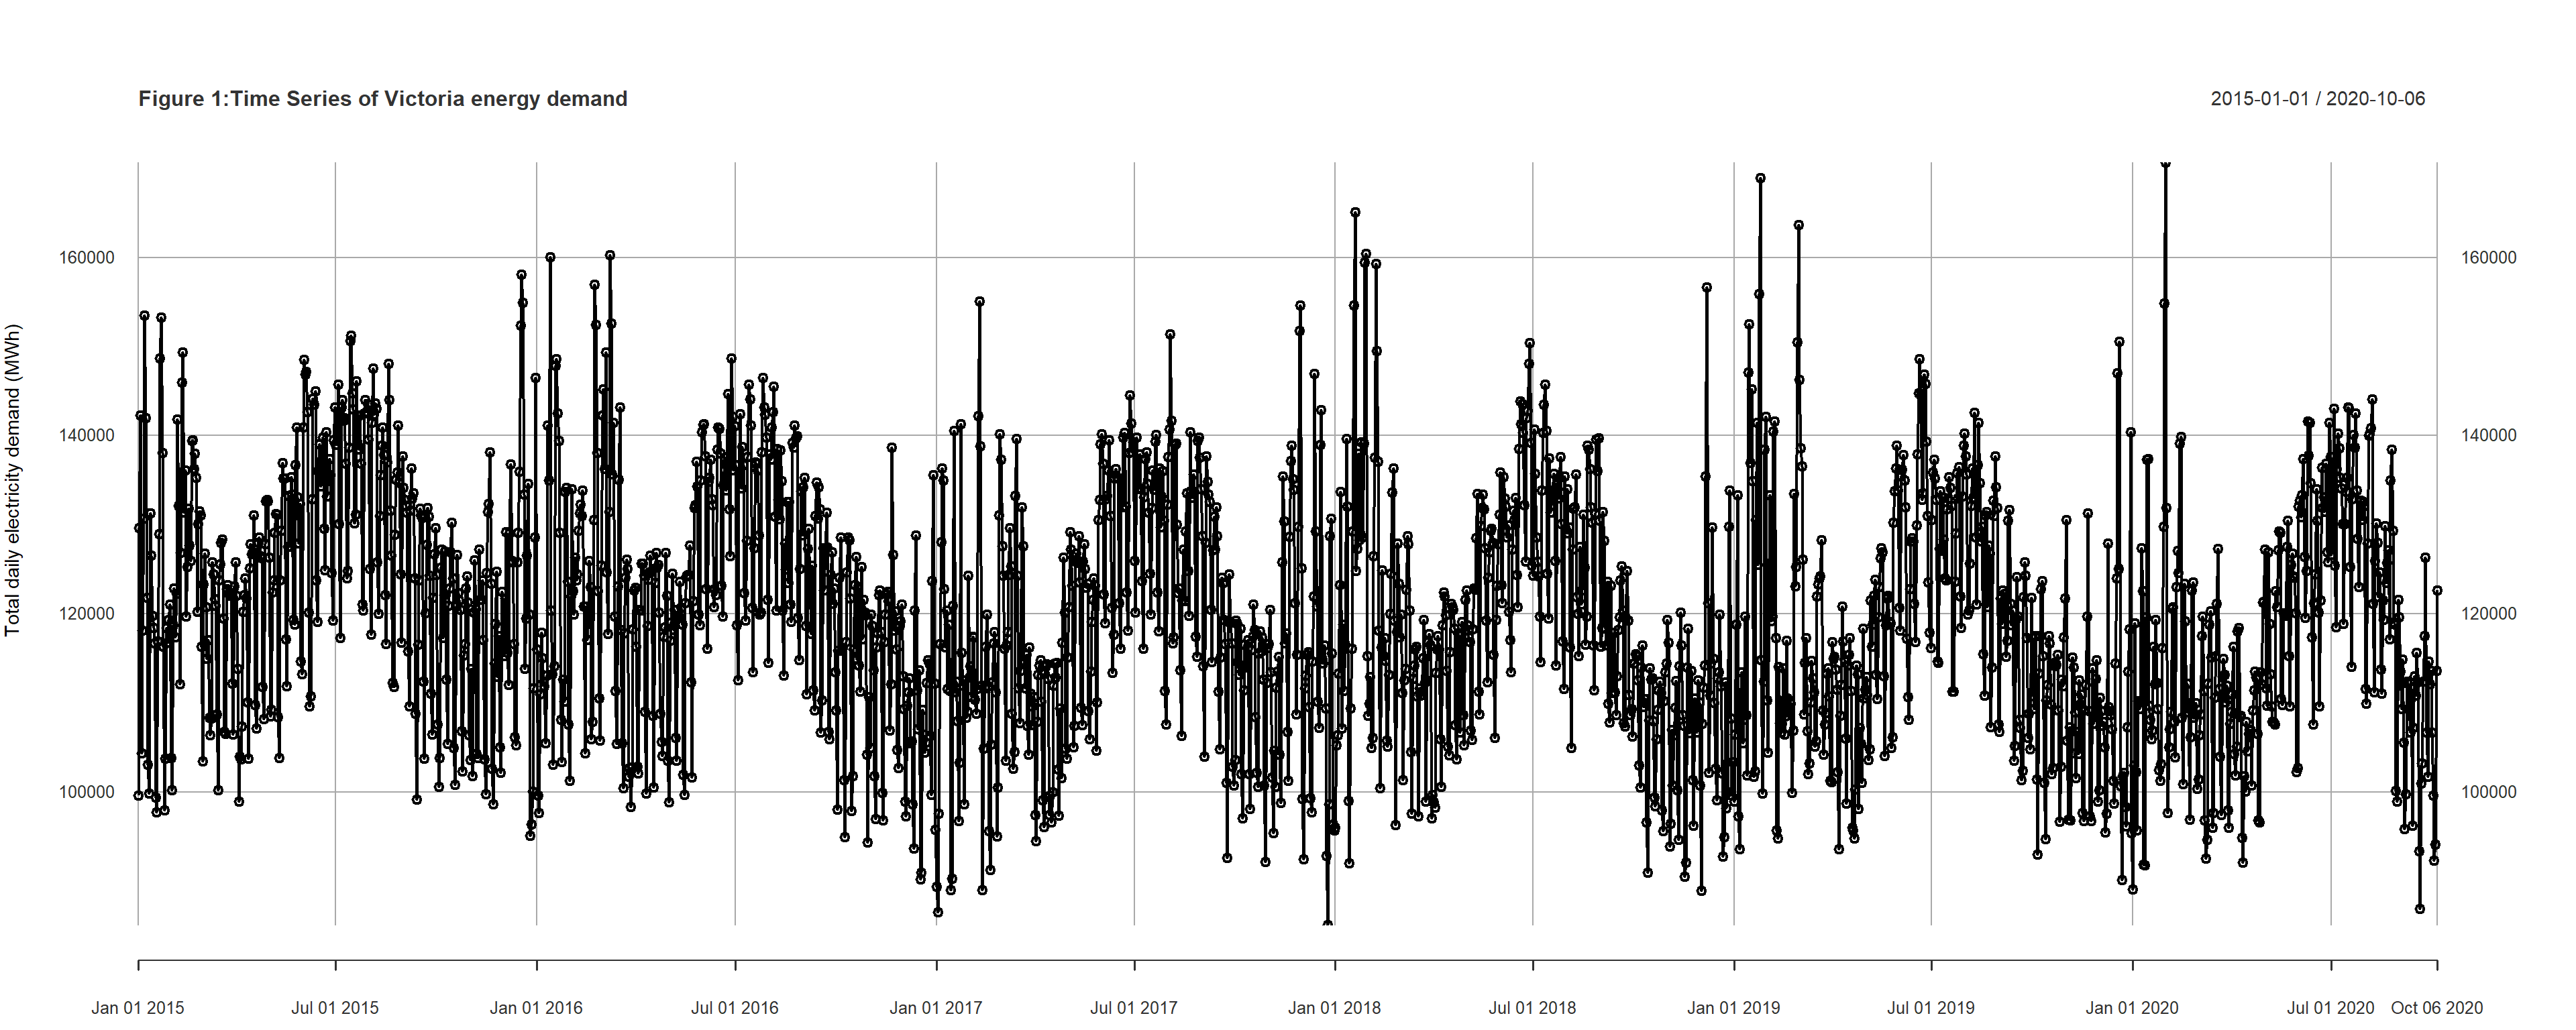
\includegraphics{Final_proj_files/figure-latex/unnamed-chunk-3-1} \end{center}
\n

\hypertarget{import-and-analyse-dataset-1}{%
\subsection{2.2 Import and Analyse
Dataset}\label{import-and-analyse-dataset-1}}

\hypertarget{data-transformations}{%
\section{3. Data transformations}\label{data-transformations}}

\hypertarget{model-specification}{%
\section{4. Model specification}\label{model-specification}}

\hypertarget{parameter-estimation}{%
\section{5. Parameter Estimation}\label{parameter-estimation}}

\hypertarget{model-diagnostics}{%
\section{6. Model Diagnostics}\label{model-diagnostics}}

\hypertarget{conclusion}{%
\section{7. Conclusion}\label{conclusion}}

\hypertarget{references}{%
\section{8. References}\label{references}}

\end{document}
